%%%%%%%%%%%% Attribution %%%%%%%%%%%%
% This template was created by 
% Chuck F. Rocca at WCSU and may be
% copied and used freely for 
% non-commercial purposes.
% 10-17-2021
%%%%%%%%%%%%%%%%%%%%%%%%%%%%%%%%%%%%%

%%%%%%% Start Document Header %%%%%%%
% In creating a new document
% copy and paste the header 
% as is.
%%%%%%%%%%%%%%%%%%%%%%%%%%%%%%%%%%%%%

\documentclass[12pt]{article}

%%%% Header Information %%%%
    %%% Document Settings %%%%
    \usepackage[utf8]{inputenc}
    \usepackage[
        twoside,
        top=1in,
        bottom=0.75in,
        inner=0.5in,
        outer=0.5in
    ]{geometry}
    \pagestyle{myheadings}

%%%% Additional Commands to Load %%%%
    \usepackage{tcolorbox}
    \tcbuselibrary{skins}
    \usepackage{minted}
    \usepackage{color}
    \usepackage{tikz}
    \usetikzlibrary{calc}
    \usepackage{tabularx,colortbl}
    \usepackage{amsfonts,amsmath,amssymb}
    \usepackage{titling}
    \usepackage{mathrsfs}
    \usepackage{calc}
    \usepackage{xepersian}

%%%% Commands to Define Homework Boxes %%%%
%%%% Box Definition %%%%
    \newtcolorbox{prob}[1]{
    % Set box style
        sidebyside,
        sidebyside align=bottom,
    % Dimensions and layout
        width=\textwidth,
        toptitle=2.5pt,
        bottomtitle=2.5pt,
        righthand width=0\textwidth,
    % Coloring
        colbacktitle=gray!30,
        coltitle=black,
        colback=white,
        colframe=white,
    % Title formatting
        title={
            #1 \hfill نمره:\phantom{WWWW}
        },
        fonttitle=\large\bfseries
    }

%%%% Environment Definition %%%%
    \newenvironment{problem}[1]{
        \begin{prob}{#1}
    }
    {
        \tcblower
        \centering
        \vspace{\baselineskip}
        \end{prob}
    }



%%%% Document Information %%%%
    \title{تکلیف سری پنجم کنترل دیجیتال}
    \date{نیسمال دوم 1402-1403}
    \author{استاد درس : دکتر طالبی}

%%%%%%% End Document Header %%%%%%%


%%%% Begin Document %%%%
% note that the document starts with
% \begin{document} and ends with
% \end{document}
%%%%%%%%%%%%%%%%%%%%%%%%
\settextfont{BNAZANIN.TTF}

\begin{document}

%%%% Format Running Header %%%%%
\markboth{\theauthor}{\thetitle}

%%%% Insert the Title Information %%%
% \maketitle


%%%% General Description of the Document %%%%
\begin{figure}[htbp]
    \centering
    
\includegraphics[width=\linewidth]{Header.png}
    % \caption{Caption}
    % \label{fig:enter-label}
\end{figure}


%%%% Introduction to the General Template %%%%
\section{بخش اجباری}
    \begin{problem}{سوال اول}
    	(برنامه ریزی) جدول زیر سه پروسه را به همراه پریود تکرار، 
    	\lr{deadline}
    	نسبی و بدترین حالت زمان اجرا آنها نشان می‌دهد.
    	\centering
    	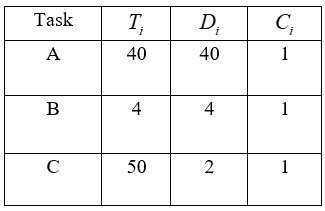
\includegraphics[scale=1]{Resources/1.png}
    	
    	\raggedright
    	الف) مجموع ضرایب استفاده \lr{CPU} را محاسبه کنید.
    	
    	ب) آیا مجموعه \lr{Task} فوق با الگوریتم زمان بندی \lr{EDF} برنامه پذیر هستند؟
    	
    	ج) سوال (ب) را با الگوریتم زمان بندی 
    	\lr{DM}
    	و
    	\lr{RM}
    	تکرار کنید.

    \end{problem}
    
    \begin{problem}{سوال دوم}
    	(برنامه ریزی) مجموعه 
    	\lr{Task}
    	زیر داده شده است:
    	
    	\centering
    	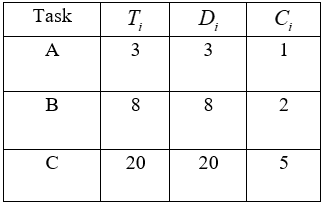
\includegraphics[scale=1]{Resources/2.png}
    	
    	\raggedright
    	الف)نشان دهید که محموعه 
    	\lr{Task}
    	فوق تحت الگوریتم
    	\lr{RM}
    	قابل برنامه ریزی است.
    	
    	ب)کوچکترین پریود 
    	\lr{Task B}
    	را که محموعه 
    	\lr{Task}
    	فوق تحت الگوریتم 
    	\lr{RM}
    	قابل برنامه ریزی است را پیدا کنید. 
    
    \end{problem}
    
\end{document}
